\documentclass{beamer}
\usepackage[slovene]{babel}
\usepackage[utf8]{inputenc}
\usepackage{graphicx}
\usepackage{float}
\usepackage{amssymb}
\usepackage{amsmath}
\usepackage{listings}
\lstset{ %
  basicstyle=\tiny\ttfamily,        % the size of the fonts that are used for the code
  tabsize=2,                       % sets default tabsize to 2 spaces
}
\usepackage{epstopdf}
\usepackage{mathtools}
%za absolutne
\DeclarePairedDelimiter\abs{\lvert}{\rvert}%

% za stolpce
\makeatletter
\newcommand{\Spvek}[2][r]{%
  \gdef\@VORNE{1}
  \left(\hskip-\arraycolsep%
    \begin{array}{#1}\vekSp@lten{#2}\end{array}%
  \hskip-\arraycolsep\right)}

\def\vekSp@lten#1{\xvekSp@lten#1;vekL@stLine;}
\def\vekL@stLine{vekL@stLine}
\def\xvekSp@lten#1;{\def\temp{#1}%
  \ifx\temp\vekL@stLine
  \else
    \ifnum\@VORNE=1\gdef\@VORNE{0}
    \else\@arraycr\fi%
    #1%
    \expandafter\xvekSp@lten
  \fi}
\makeatother
\DeclarePairedDelimiter{\ceil}{\lceil}{\rceil}
    \beamertemplatenavigationsymbolsempty
    \usetheme[progressbar=frametitle]{metropolis}
\title{Surface Simplification}
    \subtitle{Computational Topology \\
Faculty of Computer and Information Science\\
University of Ljubljana}
\author{Sven Cerk, Miha Eleršič, Mitja Rozman}
\date{6. junij 2017}

\begin{document}

\frame{\titlepage}

\begin{frame}
\frametitle{Project Goal}
\begin{itemize}
    \item{Implement an algorithm for simplifying surface triangulations}
\end{itemize}
\vspace{1cm}
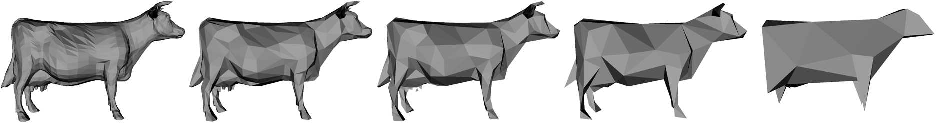
\includegraphics[width=\textwidth]{img/krava.pdf}
\end{frame}

\begin{frame}
\frametitle{Algorithm idea}
\begin{itemize}
    \item{Iteratively contract edges which minimally affect the overall shape}
    \item{Edge is chosen according to an error function}
\end{itemize}
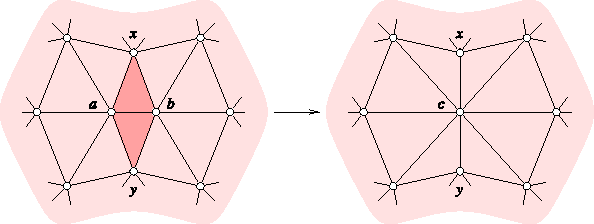
\includegraphics[width=\textwidth]{img/drawing.pdf}
\end{frame}

\begin{frame}
\frametitle{Error function}
\begin{itemize}
  \item{For each edge we compute the point to which this edge will contract}
  \item{The error of this point is calculated as the sum of squared distances to the planes spanned by adjacent triangles}
\end{itemize}
\end{frame}

\begin{frame}
\frametitle{Implementation}
\begin{itemize}
  \item{The edges are stored in a priority queue, ordered on the error of the point that replaces them}
  \item{Each iteration we contract the edge from the top the priority queue}
  \item{After contracting we discard all the adjacent edges, recompute their error and reinsert them in the priority queue}
  \item{Repeat until the number of triangles is sufficiently low}
\end{itemize}
\end{frame}

\begin{frame}
\frametitle{Demo - 5200}
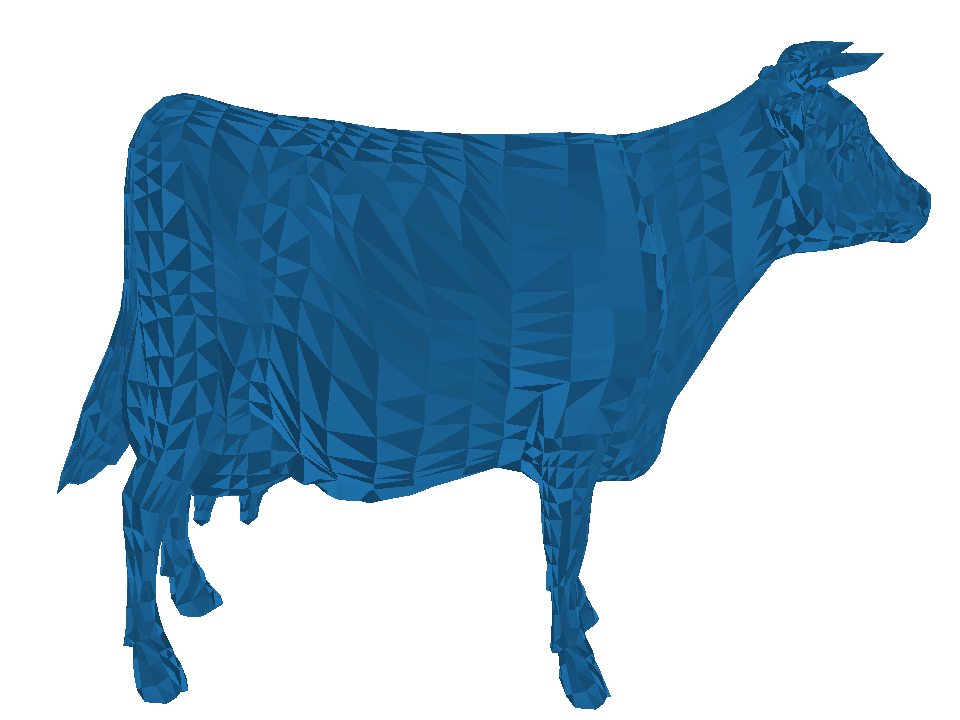
\includegraphics[width=\textwidth]{img/kravaVSE.pdf}
\end{frame}


\begin{frame}
\frametitle{Demo - 2000}
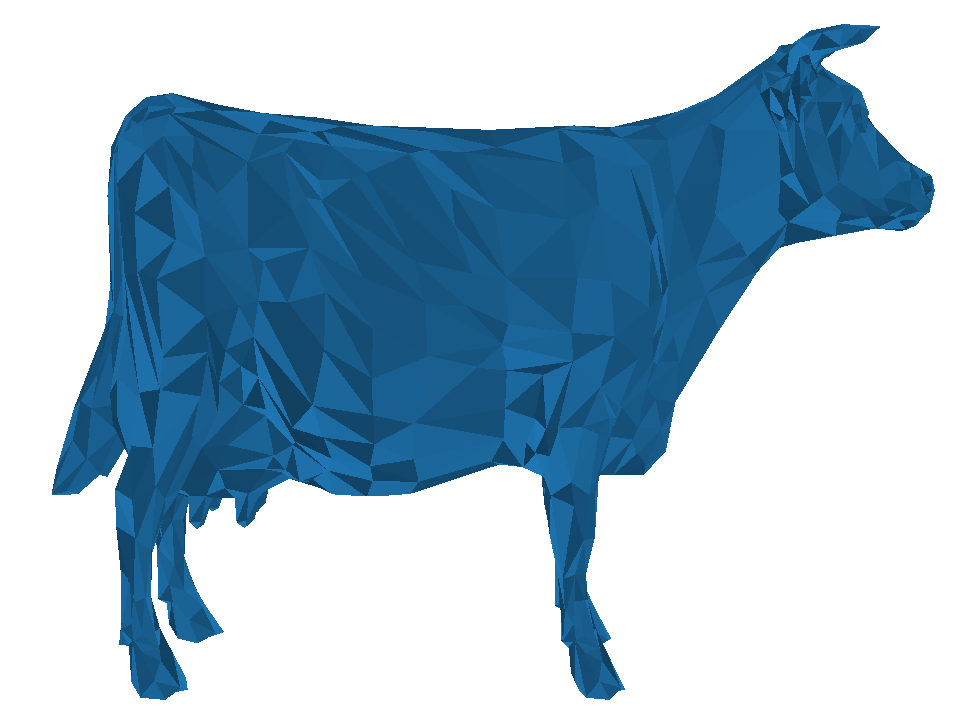
\includegraphics[width=\textwidth]{img/krava2000.pdf}
\end{frame}


\begin{frame}
\frametitle{Demo - 500}
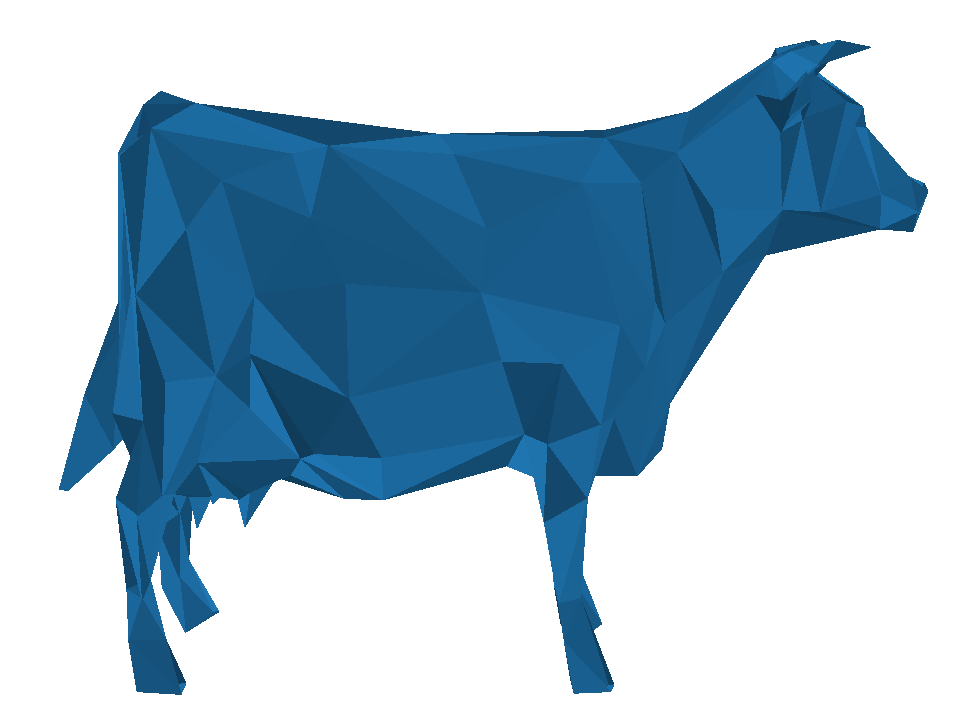
\includegraphics[width=\textwidth]{img/krava500.pdf}
\end{frame}

\begin{frame}
\frametitle{Demo - 200}
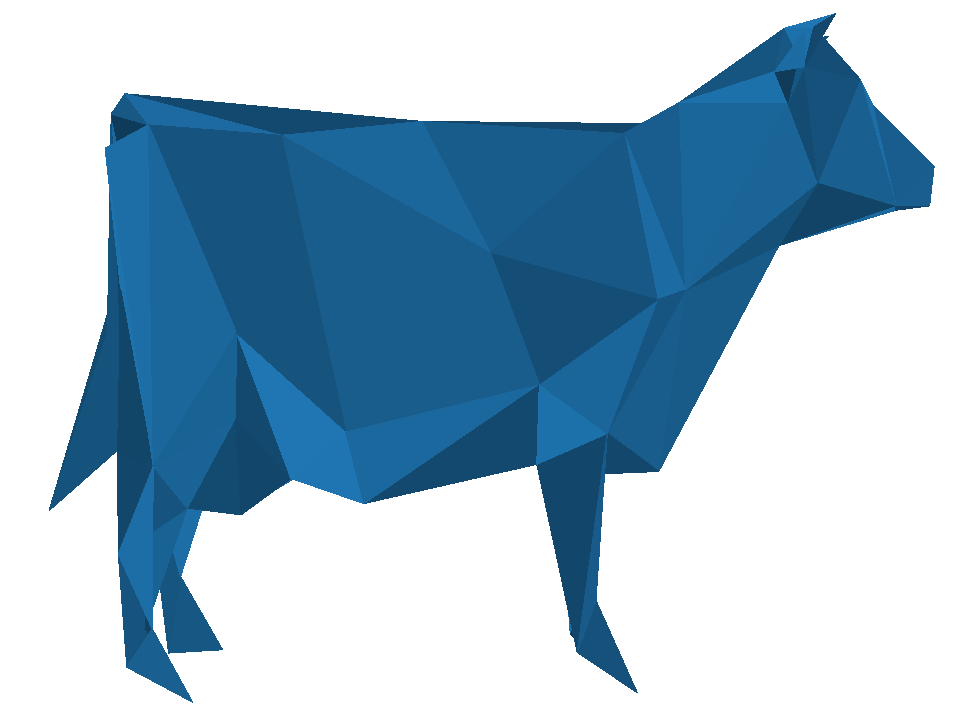
\includegraphics[width=\textwidth]{img/krava200.pdf}
\end{frame}


\begin{frame}
\frametitle{Demo - 60}

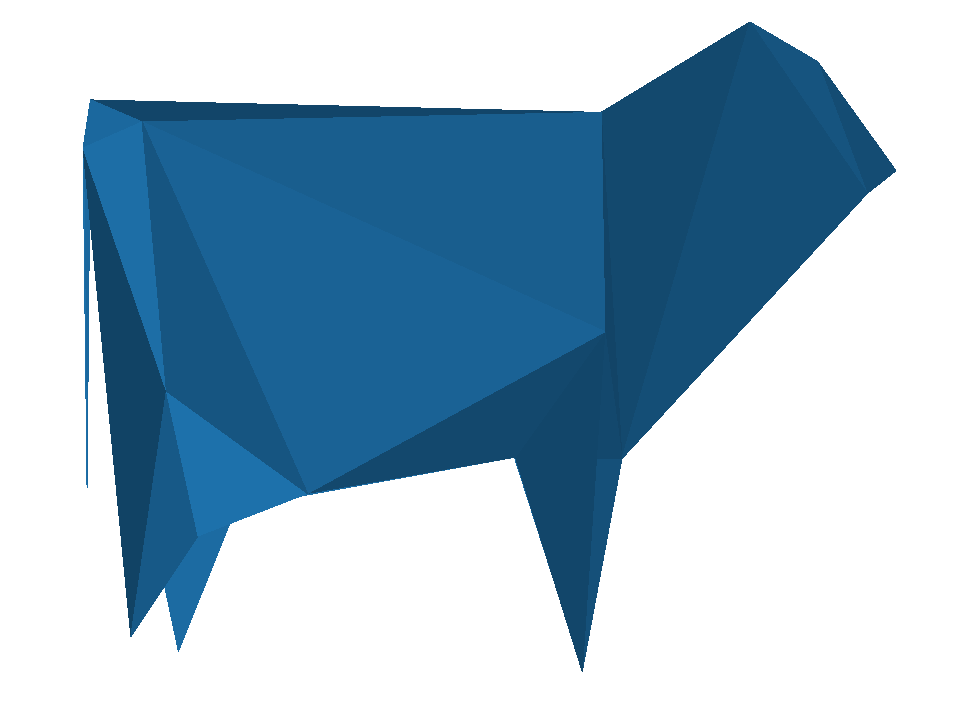
\includegraphics[width=\textwidth]{img/krava60.pdf}
\end{frame}




\end{document}
%---------------------------------------------------------




